%================================================================================
%       Safety Critical Systems Club - Data Safety Initiative Working Group
%================================================================================ 
%                       DDDD    SSSS  IIIII  W   W   GGGG
%                       D   D  S        I    W   W  G   
%                       D   D   SSS     I    W W W  G  GG
%                       D   D      S    I    WW WW  G   G
%                       DDDD   SSSS   IIIII  W   W   GGG
%================================================================================
%               Data Safety Guidance Document - LaTeX Source File
%================================================================================
%
% Description:
%   This is the main document file, it simply marks the beginning and end of the
%   document and 'includes' each of the document sections, in the required order.
%
% Notes:
%   The actual document content is contained in the files that are 'included' by 
% this one.
%
%================================================================================

%\documentclass[letterpaper,10pt]{book}
%\usepackage[hyperref]{../dsiwg}
\def\withCovers{}
\def\withBlueHyperlinks{}
\def\withChangebars{} %Markers are \cbstart and \cbend. Remember to delete markers for previous changes before starting update.
\def\withToDo{} %Post-it note in the margin to highlight issues to be resolved before publication

%================================================================================
%       Safety Critical Systems Club - Data Safety Initiative Working Group
%================================================================================
%                       DDDD    SSSS  IIIII  W   W   GGGG
%                       D   D  S        I    W   W  G   
%                       D   D   SSS     I    W W W  G  GG
%                       D   D      S    I    WW WW  G   G
%                       DDDD   SSSS   IIIII  W   W   GGG
%================================================================================
%               Data Safety Guidance Document - LaTeX Source File
%================================================================================
%
% Description:
%   This file contains all of the LaTeX macros to control the template for the
%   Data Safety Guidance Document.
%
% !!WARNING!!
%   CHANGING THE CONTENT OF THIS PARTICULAR FILE CAN SERIOUSLY AFFECT THE
%   APPEARANCE AND LAYOUT OF THE GENERATED DOCUMENT, SO PLEASE BE CAREFUL.
%
% Label formats:
%   bkm: ==>      Reference to another part of this document
%   citation: ==> Reference to an external document listed in bibTex
%   fig: ==>      Reference to a figure within this document
%   ftn: ==>      Reference to a footnote within this document
%   tab: ==>      Reference to a table within this document
%
% Notes:
%   All commands, styles, colours, etc. defined within this template shall begin
%   with the prefix of 'dsiwg' to distinguish them from built-in TeX keywords or
%   those in third-party packages.
%

%================================================================================
%Version 2.0 was US Letter paper with a default font of 10pt, this may change
%================================================================================
\documentclass[letterpaper,10pt,twoside]{article}

% May be able to remove in future, when pdflatex default output becomes pdf 1.7 or greater
\pdfminorversion=7 % Required to read darkknowns.pdf at v1.7, but default from pdflatex is 1.5

%================================================================================
%Set the default font family and series for the document to 'Open Sans Light'
%================================================================================
\usepackage[utf8]{inputenc}
\usepackage[T1]{fontenc}
\usepackage[default,defaultsans]{opensans}% On TeXLive 2018, "default" was enough. Need "defaultsans" from TeXLive 2019
\usepackage{textcomp}           %Required for complete font support
\renewcommand{\seriesdefault}{l}% Select Open Sans Light as the default font

%================================================================================
%Load all other required packages
%================================================================================
\usepackage[
  title,%
  titletoc%
]{appendix}                     %Used to add appendices into the ToC
\usepackage{tocvsec2}           %Allow suppression of selected entries within TOC
%--------------------------------------------------------------------------------
\usepackage{calc}               %Used for infix calculations, e.g. column widths 
\usepackage{color}              %Used to set foreground and background colours
\usepackage{colortbl}           %Used to add colour to LaTeX tables
\usepackage{enumitem}           %Used to control the different list environments
\usepackage{fancyhdr}           %Used to define the header and footer layout
\usepackage{float}              %Used to force specific placement of images
\usepackage[hang]{footmisc}     %Used to make footnotes a numbered list
%--------------------------------------------------------------------------------
\ifx\withChangebars\undefined
% Shortcut to create version without changebars
\newcommand{\cbstart}{}
\newcommand{\cbend}{}
\else
\usepackage{changebar}          %Markers are \cbstart and \cbend.
\fi
%--------------------------------------------------------------------------------
\usepackage[
  dvips =false,%
  pdftex=false,%
  vtex  =false,%
  bottom=1.5cm,%
  left  =2.5cm,%
  right =2.5cm,%
  top   =1.5cm,%
  head  =18pt  %
]{geometry}                     %Used to set-up the page layout and margins
%--------------------------------------------------------------------------------
\usepackage[pdftex]{graphicx}   %Used to insert diagrams into the document
%--------------------------------------------------------------------------------
%\usepackage[
%  acronyms,%
%  toc
%]{glossaries}                   %Used to create and print the glossary - very sensitive to package order
%--------------------------------------------------------------------------------
\usepackage[none]{hyphenat}     %Used to prevent hyphenation in the document
\usepackage{longtable}          %Used for tables that break across pages
\usepackage{caption}            %Adds longtable* which is needed to create longtables that do not increment the table counter
\usepackage{multirow}           %Used to allow multiple row spanning in tables
\usepackage{pifont}             %Used to print ZipfDingbats characters (\ding)
\usepackage[many]{tcolorbox}    %Used to place coloured boxes around text

\ifx\withToDo\undefined
% Shortcut to create version without todo notes
\newcommand{\todo}[1]{}
\newcommand{\listoftodos}{}
\else
\usepackage[textwidth=2cm]{todonotes} %Allows multi-line markup of text which needs to be amended/reviewed ie, yellow highlighter
\fi

\usepackage{pdfpages}           %Handy way to insert covers
\usepackage{wrapfig}            %Wrap text around a figure
\usepackage{imakeidx}

\usepackage[framemethod=tikz]{mdframed}           %Put text in a box that can break across pages
\newmdenv[frametitle=Response of the AI,%
  roundcorner=10pt,
linewidth=2pt]{aibox} % Environment to display AI-generated text
%--------------------------------------------------------------------------------
% Set up indexes.
% Page style gets upset for indexes, unless we set it explicitly
%
\makeindex[name=locationidx,title=Index of Locations,intoc]
\makeindex[title=Index,intoc]
\indexsetup{
  othercode={%
    \thispagestyle{Standard}%
  }
}
% Break long URLs
\usepackage{url}
\def\UrlBreaks{\do\/\do-}
\usepackage{breakurl}
%--------------------------------------------------------------------------------
%The hyperref is best loaded last to avoid conflicts, e.g. with glossaries
%TGR: the glossaries package documentation says it must be loaded after the hyperref package.
%--------------------------------------------------------------------------------
\ifx\withBlueHyperlinks\undefined
\usepackage[                    %Could use \hypersetup but easier to do it here
  breaklinks,%
  bookmarksnumbered,%
  pdftex,%
  pdfpagelayout=OneColumn,% "OneColumn" produces a single continous scrolling viewer display; was previously set to "TwoColumnRight" for two pages side by side with odd pages on the right.
  pdfpagelabels,%
  hidelinks,% Make the links visually just normal text
  linktoc=page
]{hyperref}                     %Creates property fields & hyperlinks in the PDF - For details see http://www.tug.org/applications/hyperref/manual.html#x1-110003.7
\else
\usepackage[                    %Could use \hypersetup but easier to do it here
  bookmarksnumbered,%
  pdftex,%
  pdfpagelayout=OneColumn,% "OneColumn" produces a single continous scrolling viewer display; was previously set to "TwoColumnRight" for two pages side by side with odd pages on the right.
  pdfpagelabels,%
  colorlinks=true,% Select coloured text, rather than coloured boxes around links
  linkcolor=blue,          % color of internal links (change box color with linkbordercolor)
  citecolor=blue,        % color of links to bibliography
  filecolor=blue,      % color of file links
  urlcolor=blue,           % color of external links
  linktoc=page
]{hyperref}                     %Creates property fields & hyperlinks in the PDF - For details see http://www.tug.org/applications/hyperref/manual.html#x1-110003.7
\fi

%================================================================================
%Create some new commands to quickly change local font style
%================================================================================
\DeclareRobustCommand\ebseries{\fontseries{eb}\selectfont}
\DeclareRobustCommand\sbseries{\fontseries{sb}\selectfont}
\DeclareRobustCommand\ltseries{\fontseries{l}\selectfont}
\DeclareRobustCommand\clseries{\fontseries{cl}\selectfont}
\DeclareRobustCommand\regseries{\fontseries{m}\selectfont}

\DeclareTextFontCommand{\dsiwgTextEB}{\ebseries}    %Extra-Bold typeface
\DeclareTextFontCommand{\dsiwgTextSB}{\sbseries}    %Semi-Bold typeface
\DeclareTextFontCommand{\dsiwgTextLT}{\ltseries}    %Light typeface
\DeclareTextFontCommand{\dsiwgTextCL}{\clseries}    %Condensed-light typeface
\DeclareTextFontCommand{\dsiwgTextREG}{\regseries}  %Regular typeface

\DeclareTextFontCommand{\dsiwgTextBF}{\sbseries}    %What 'bold-face' looks like
\DeclareTextFontCommand{\dsiwgTextIT}{\itshape}     %What 'italic' looks like

%
%Create a new environment to change the font shape for large blocks of text.
%Using begin/end is more obvious than just using one of the above commands.
%
\newenvironment{dsiwgBold}{\sbseries}{}
\newenvironment{dsiwgItalic}{\itshape}{}

%
%Unfortunately the Open Sans font doesn't support a typewriter style in 'light'
%series, so we have to declare a special version to avoid warnings when compiling
%the document.
%
% For manual use:
\newcommand{\dsiwgTextTT}[1]{\usefont{T1}{cmtt}{m}{n}{#1}}
%
% To make \url use the right font
% We need these next two lines, but they fail to load T1/cmtt/m/n, so we put up with warning for now
%\DeclareFontFamily{T1}{cmtt}{\hyphenchar\font=-1}
%\DeclareFontShape{T1}{cmtt}{l}{n}{ <-> ssub * cmtt/m/n }{}

%
%Set the character to be used for the check box on the ODR forms, etc.
%
\newcommand{\dsiwgCheckBox}{\large{\ding{111}}}

%================================================================================
%Space things out a bit
%================================================================================
\linespread{1.2}

%================================================================================
%Mark intentionally blank pages as such
%================================================================================
\makeatletter
\def\dsiwg@intblankpage{%
	\clearpage% this line has no effect if invoked from dsiwg@cleardoublepage
	\null\vfil
	\centerline{This page is intentionally blank}%
	\newpage
        \phantomsection% Required to move page counter in \label associated with following \section point to correct page
}

\def\dsiwg@cleardoublepage{%
    \clearpage%needed here so that we test AFTER the page throw
	\ifodd\c@page\else
		\dsiwg@intblankpage
	\fi
}
\let\cleardoublepage=\dsiwg@cleardoublepage
\makeatother

%================================================================================
%Define the colours to be used for this template style
%================================================================================
%
%Document accent colour for headings, etc. (set to a shade of blue)
%
%\definecolor{dsiwgAccentColour}{RGB}{233,33,33} %Red - v2.0
\definecolor{dsiwgAccentColour}{RGB}{0,102,255} %Blue - v3.0
\definecolor{dsiwgDimColour}{RGB}{51,153,255} %Pale Blue - v3.6
%
%Colours to be used for the objectives list box at the start of each section 
%
%\definecolor{dsiwgObjectiveBackgroundColour}{RGB}{233,15,12}
%\definecolor{dsiwgObjectiveFrameColour}{RGB}{233,132,132}

%================================================================================
%Assign colours to the various document elements
%================================================================================
%
%Set the colours for all of the section headings
%
\colorlet{dsiwgSectionColour}{dsiwgAccentColour}
\colorlet{dsiwgSubSectionColour}{dsiwgSectionColour}
\colorlet{dsiwgSubSubSectionColour}{dsiwgSectionColour}
\colorlet{dsiwgParagraphColour}{dsiwgSectionColour}

%
%Set the colours for all four levels of enumerated list
%
\preto\labelenumi{\color{dsiwgAccentColour}}
\preto\labelenumii{\color{dsiwgAccentColour}}
\preto\labelenumiii{\color{dsiwgAccentColour}}
\preto\labelenumiv{\color{dsiwgAccentColour}}

%
%Set the colours for all four levels of bulleted list
%Also make the top-level bullet large
%
%\preto\labelitemi{\large\color{dsiwgAccentColour}}
\renewcommand\labelitemi{\large\color{dsiwgAccentColour}$\bullet$}
\preto\labelitemii{\color{dsiwgAccentColour}}
\preto\labelitemiii{\color{dsiwgAccentColour}}
\preto\labelitemiv{\color{dsiwgAccentColour}}

%
%Set the background and edge colours for the quotes
%
\definecolor{dsiwgQuoteBackColour}{gray}{0.95}
\definecolor{dsiwgQuoteFrameColour}{gray}{0.65}

%
%Set up colour for TBD highlighting - stuff to be fixed prior to release
%
%\definecolor{dsiwgTbdColour}{rgb}{1,1,0}
%\newcommand{\dsiwgTbd}[1]{{\todo[color=dsiwgTbdColour,inline]{#1}}}
\setlength{\marginparwidth}{2cm}%Keeps todo note in margin

%================================================================================
% Enhancements to allow fixed width columns, with left, centred or right aligned
% text (the usual m option only allows justified, creating underfull hboxes)
%================================================================================
\newcolumntype{L}[1]{>{\raggedright\let\newline\\\arraybackslash\hspace{0pt}}m{#1}}
\newcolumntype{C}[1]{>{\centering\let\newline\\\arraybackslash\hspace{0pt}}m{#1}}
\newcolumntype{R}[1]{>{\raggedleft\let\newline\\\arraybackslash\hspace{0pt}}m{#1}}

%================================================================================
%Format the quotes at the beginning of each section. This takes two arguments:
%1) the quote, 2) the author (can be empty if the quote is not attributed)
%================================================================================
\newcommand\dsiwgSectionQuote[2]{
  \begin{center}
    \begin{tcolorbox}
      [ boxsep=0mm,
        colback=dsiwgQuoteBackColour,
        colframe=dsiwgQuoteFrameColour,
        bottomrule=0mm,
        toprule=0mm,
        leftrule=4pt,
        rightrule=4pt,
        sharp corners,
        width=0.89\linewidth
      ]
      \begin{center}
        \dsiwgTextIT{#1}
        \ifx&#2&
          %Empty field, do nothing.
        \else
          \\\dsiwgTextBF{\dsiwgTextIT{{#2}}}
        \fi
      \end{center}
    \end{tcolorbox}
  \end{center}
}

\newcommand\dsiwgColumnWidth[1]{#1\linewidth-2\tabcolsep-1.25\arrayrulewidth}

%================================================================================
%Create a new environment for the objectives box used at the start of a section.
%================================================================================
\usetikzlibrary{shadings}
\newenvironment{dsiwgObjectiveList}{\begin{enumerate}[label=\arabic*.\color{white}] \color{white} \sbseries \slshape}{\end{enumerate}}
\tcolorboxenvironment{dsiwgObjectiveList}
{%
  enhanced jigsaw,
  boxsep=0mm,
  colframe=dsiwgObjectiveFrameColour,
  boxrule=4pt,
  sharpish corners,
  drop shadow=black,
  interior style={left color=dsiwgObjectiveBackgroundColour!95!white,right color=dsiwgObjectiveBackgroundColour!95!white,middle color=dsiwgObjectiveBackgroundColour!75!white,opacity=0.75},
  width=0.89\textwidth
}

%================================================================================
%Set-up the table header colour scheme and fonts
%================================================================================

%
%There are so many ``centered'' or ragged entries that it was worth adding
%special commands for these.
%
\newcommand\TableHeadColour[1]{\cellcolor{dsiwgAccentColour}{\ebseries\small\color{white}{#1}}}
\newcommand\TableHeadColourC[1]{\centering\TableHeadColour{#1}}% Version with contents centred
\newcommand\TableHeadColourR[1]{\raggedleft\TableHeadColour{#1}}% Version with contents raggedleft
\newcommand\TableDimColour[1]{\cellcolor{dsiwgDimColour}{\ebseries\small\color{white}{#1}}}
%
%Special versions with contents centred, and \\ bug correction for right hand column
%Modification of above form doesn't work - the position of the \arraybslash seems to be critical
%
\newcommand\TableHeadColourCX[1]{\cellcolor{dsiwgAccentColour}\centering\arraybslash{\ebseries\small\color{white}#1}}
\newcommand\TableDimColourCX[1]{\cellcolor{dsiwgDimColour}\centering\arraybslash{\ebseries\small\color{white}#1}}

%
%Set table fonts here to avoid setting on every table cell
%
\makeatletter
% Thanks to Axel Sommerfeldt [2007/01/07] for this macro:
\providecommand*\AtBeginEnvironment[1]{%
  \@ifundefined{#1}%
               {\@latex@error{Environment #1 undefined}\@ehc
                 \@gobble}%
               {\@ifundefined{ABE@env@#1}%
                 {\expandafter\let\csname ABE@env@#1\expandafter\endcsname
                   \csname #1\endcsname
                   \expandafter\let\csname ABE@hook@#1\endcsname\@empty
                   \@namedef{#1}{\@nameuse{ABE@hook@#1}\@nameuse{ABE@env@#1}}}%
                 {}%
                 \expandafter\g@addto@macro\csname ABE@hook@#1\endcsname}}
\@onlypreamble\AtBeginEnvironment
\makeatother

%
%Whenever we create a longtable set the font size
%
\AtBeginEnvironment{longtable}{\small}

%================================================================================
%Set-up some text styles
%================================================================================

%
%Colour for numbers in section, subsection and subsubsection
%
\newcommand\textstyleNumberingSymbols[1]{\textsf{\textcolor{dsiwgAccentColour}{#1}}}
\newcommand\textstyleBulletSymbols[1]{{\normalsize\selectfont\textsf{\textbf{\textcolor{dsiwgAccentColour}{#1}}}}}
\newcommand\textstyleCitation[1]{\textit{#1}}
\newcommand\textstyleFootnoteanchor[1]{{\normalsize\selectfont\textsf{\textmd{\textsuperscript{#1}}}}}

%================================================================================
%Set up spacing heading/section spacing, as per original Version 2.0 template
%================================================================================
\makeatletter
  %Heading Level 1
  \renewcommand\section%
  {%
    \@startsection{section}{1}{0pt}{4pt}{0.1mm}%
    {\cleardoublepage\pagestyle{Standard}\thispagestyle{FirstPage}\raggedright\normalfont\LARGE\regseries\normalcolor\color{dsiwgSectionColour}}%
  }

  %Heading Level 2
  \renewcommand\subsection%
  {%
    \@startsection{subsection}{2}{0pt}{18pt}{0.1mm}%
    {\normalfont\Large\regseries\normalcolor\color{dsiwgSubSectionColour}}%
  }

  %Heading Level 3
  \renewcommand\subsubsection%
  {%
    \@startsection{subsubsection}{3}{0pt}{18pt}{0.1mm}%
    {\normalfont\large\regseries\normalcolor\color{dsiwgSubSubSectionColour}}%
  }

  %Heading Level 4
  \renewcommand\paragraph%
  {%
    \@startsection{paragraph}{4}{0pt}{18pt}{0.1mm}%
    {\normalfont\normalsize\regseries\normalcolor\color{dsiwgParagraphColour}}%
  }
	
\makeatother

%A Non-numbered version of paragraph
\newcommand\nonumparagraph[1]{{\normalfont\normalsize\regseries\normalcolor\textcolor{dsiwgParagraphColour}{#1}}}


%================================================================================
%Set-up the headings and outline numbering
%================================================================================
\makeatletter
  \renewcommand\@seccntformat[1]{\csname @textstyle#1\endcsname{\csname the#1\endcsname}\csname @distance#1\endcsname}
  \setcounter{secnumdepth}{4}
  \newcommand\@distancesection{\hspace{1cm}}
  \newcommand\@textstylesection[1]{\protect\makebox[0cm][l]{\textstyleNumberingSymbols{#1}}}
  \newcommand\@distancesubsection{\hspace{1.27cm}}
  \newcommand\@textstylesubsection[1]{\protect\makebox[0cm][l]{\textstyleNumberingSymbols{#1}}}
  \newcommand\@distancesubsubsection{\hspace{1.27cm}}
  \newcommand\@textstylesubsubsection[1]{\protect\makebox[0cm][l]{\textstyleNumberingSymbols{#1}}}
  \newcommand\@distanceparagraph{\hspace{1.52cm}}\newcommand\@textstyleparagraph[1]{\protect\makebox[0cm][l]{\textstyleNumberingSymbols{#1}}}
\makeatother

\makeatletter
  \newcommand\arraybslash{\let\\\@arraycr}
\makeatother
\raggedbottom

%================================================================================
%Set-up the paragraph styles
%================================================================================
\renewcommand\familydefault{\sfdefault}

\newenvironment{styleTextbody}{\setlength\leftskip{0cm}\setlength\rightskip{0cm}\setlength\parindent{0cm}\setlength\parfillskip{0pt plus 1fil}\setlength\parskip{0.349cm plus 0.0349cm}\leavevmode\normalfont\normalsize\normalcolor\ignorespaces}{\unskip\vspace{0cm plus 1pt}\par}

\newenvironment{styleMainTitle}{\clearpage\setcounter{page}{1}\pagestyle{FirstPageFrontMatter}
  \thispagestyle{FirstPageTitle}
  \setlength\leftskip{3.551cm}\setlength\rightskip{2cm}\setlength\parindent{0cm}\setlength\parfillskip{0pt plus 1fil}\setlength\parskip{0cm plus 1pt}\leavevmode\normalfont\huge\normalcolor\color{dsiwgAccentColour}\ignorespaces}{\unskip\vspace{0.28cm plus 0.027999999cm}\par}

\newenvironment{styleTitlePageAuthor}{\setlength\leftskip{3.551cm}\setlength\rightskip{5.001cm}\setlength\parindent{0cm}\setlength\parfillskip{0pt plus 1fil}\setlength\parskip{0cm plus 1pt}\leavevmode\normalfont\Large\normalcolor\color{dsiwgAccentColour}\ignorespaces}{\unskip\vspace{0cm plus 1pt}\par}

\newenvironment{styleTitlePageDate}{\setlength\leftskip{3.551cm}\setlength\rightskip{2cm}\setlength\parindent{0cm}\setlength\parfillskip{0pt plus 1fil}\setlength\parskip{0.28cm plus 0.027999999cm}\leavevmode\normalfont\normalsize\normalcolor\sffamily\mdseries\color{dsiwgAccentColour}\ignorespaces}{\unskip\vspace{0cm plus 1pt}\par}

\newenvironment{styleQuotation}{\setlength\leftskip{0cm plus 1fil}\setlength\rightskip{0cm plus 1fil}\setlength\parindent{0cm}\setlength\parfillskip{0pt}\setlength\parskip{0.349cm plus 0.0349cm}\leavevmode\normalfont\small\normalcolor\ignorespaces}{\unskip\vspace{0cm plus 1pt}\par}

%
%Footnote rule
%
\setlength{\skip\footins}{0.119cm}
\renewcommand\footnoterule{\vspace*{-0.018cm}\setlength\leftskip{0pt}\setlength\rightskip{0pt plus 1fil}\noindent\textcolor{black}{\rule{0.25\columnwidth}{0.018cm}}\vspace*{0.101cm}}

%================================================================================
%Define the coloured blob to go in the footer, near the page number
%================================================================================
%
%The blob itself
%
\newcommand{\blob}{\textcolor{dsiwgAccentColour}{\rule[-1em]{0.5em}{4em}}}

%
%Make it take up zero vertical space and set up header and footer offsets for it
%
\newcommand{\tlap}[1]{\mbox{\vbox to 0pt{\vss\hbox{#1}}}}
\newlength\OurHeadOffset
\setlength\OurHeadOffset{30pt}
\newlength\OurFootOffset
\setlength\OurFootOffset\OurHeadOffset
\addtolength\OurFootOffset{-1em}

%
%Then define the two footers
%
\newcommand{\leftfoot}{\tlap{\llap{\thepage\hspace{0.5em}\blob}\vspace{2em}}}
\newcommand{\rightfoot}{\tlap{\rlap{\blob\hspace{0.5em}\thepage}\vspace{2em}}}

%================================================================================
%Set-up the different page styles used within the document
%================================================================================
\fancypagestyle{FirstPageFrontCover}{\fancyhf{}
  \fancyhead[L]{}
  \fancyfoot[L]{}
  \renewcommand\headrulewidth{0pt}
  \renewcommand\footrulewidth{0pt}
  \renewcommand\thepage{}
  \vspace*{6cm}
  \pagenumbering{alph}
  \renewcommand\thepage{\alph{page}}
}
\fancypagestyle{ContinuationInsideFrontCover}{\fancyhf{}
  \fancyhead[L]{}
  \fancyfoot[L]{}
  \renewcommand\headrulewidth{0pt}
  \renewcommand\footrulewidth{0pt}
  \renewcommand\thepage{}
  \vspace*{4cm}
  \renewcommand\thepage{\alph{page}}
}
\fancypagestyle{FirstPageFrontMatter}{\fancyhf{}%Always page i, so that's a RO page
  \renewcommand\headrulewidth{0pt}
  \renewcommand\footrulewidth{0pt}
  \pagenumbering{roman}
  \renewcommand\thepage{\roman{page}}
}
\fancypagestyle{ContinuationPageFrontMatter}{\fancyhf{}
  \fancyheadoffset\OurHeadOffset% How far to put header and footer outside of text width
  \fancyfootoffset\OurFootOffset% How far to put header and footer outside of text width
  \fancyhead[LO]{}
%  \fancyhead[LE, RO]{\large\color{dsiwgAccentColour} {\rotatebox{90}{\llap{\leftmark\hspace{2em}}}}}
  \fancyfoot[LO]{}
  \fancyfoot[LE]{\leftfoot}
  \fancyfoot[RO]{\rightfoot}
  \renewcommand\headrulewidth{0pt}
  \renewcommand\footrulewidth{0pt}
  \renewcommand\thepage{\roman{page}}
}
\fancypagestyle{Standard}{\fancyhf{}
  \fancyheadoffset\OurHeadOffset% How far to put header and footer outside of text width
  \fancyfootoffset\OurFootOffset% How far to put header and footer outside of text width
  \fancyhead[LO]{}
  %\fancyhead[LE, RO]{\large\color{dsiwgAccentColour} {\rotatebox{90}{\llap{\leftmark\hspace{2em}}}}}
  \fancyfoot[LO]{}
  \fancyfoot[LE]{\leftfoot}
  \fancyfoot[RO]{\rightfoot}
  \renewcommand\headrulewidth{0pt}
  \renewcommand\footrulewidth{0pt}
  \renewcommand\thepage{\arabic{page}}
}
\fancypagestyle{FirstPageAppendix}{\fancyhf{}
  \fancyhead[LO]{\large\color{dsiwgAccentColour} [Warning: Draw object ignored]}
  \fancyhead[LE]{\large\color{dsiwgAccentColour} [Warning: Draw object ignored]}
  \fancyfoot[LO]{}
  \fancyfoot[LE]{}
  \renewcommand\headrulewidth{0pt}
  \renewcommand\footrulewidth{0pt}
  \renewcommand\thepage{\arabic{page}}
}
\fancypagestyle{FirstPageTitle}{\fancyhf{}
  \fancyhead[L]{\large\color{dsiwgAccentColour} [Warning: Draw object ignored]}
  \fancyfoot[L]{\large{\scriptsize\textcolor[rgb]{0.5019608,0.0,0.0}{MISRA internal use only}}\hfill \thepage{}}
  \renewcommand\headrulewidth{0pt}
  \renewcommand\footrulewidth{0pt}
  \renewcommand\thepage{\roman{page}}
}
\fancypagestyle{FirstPage}{\fancyhf{}
  \fancyfootoffset\OurFootOffset% How far to put header and footer outside of text width
  \fancyhead[LO,LE,RO,RE]{}
  \fancyfoot[LO,RE]{}
  \fancyfoot[LE]{\leftfoot}
  \fancyfoot[RO]{\rightfoot}
  \renewcommand\headrulewidth{0pt}
  \renewcommand\footrulewidth{0pt}}

\setlength\tabcolsep{1mm}
\renewcommand\arraystretch{1.3}
\sloppy

%================================================================================
%Utility to make it easier for us to make "section X" a hyperlink, rather than just the X
% Needed because \autoref is inconsistent in references appendices -
% Some were shown as "section M", others as "Appendix O".
% Also useful for referencing subsubsections.
%================================================================================

\newcommand{\dsiwgRef}[2]{\hyperref[#2]{#1}~\ref{#2}}

%================================================================================
% Utility to make it easier to add entries to the acronym list
%================================================================================
%\newcommand{\acrentry}[1]{\acrshort{#1}&\acrlong{#1}\\\hline}

%================================================================================
%Prevent the bibliography macros from inserting their own ``References'' heading.
%================================================================================
\patchcmd{\thebibliography}{\section*{\refname}}{}{}{}

%================================================================================
%Set-up the list of Abbreviations and Glossary
%================================================================================
% TGR moved to end
% \loadglsentries{glossary}
% Next line commented out as glossaries not yet generated by package glossaries
%\makeglossaries

%================================================================================
%Allow searching of ligatures in Adobe Reader
%================================================================================
\input{glyphtounicode}

\pdfglyphtounicode{f_f}{FB00}
\pdfglyphtounicode{f_f_i}{FB03}
\pdfglyphtounicode{f_f_l}{FB04}
\pdfglyphtounicode{f_i}{FB01}

\pdfgentounicode=1
%
% Define the tick mark for use in tables 
%
\newcommand\tick{\ding{51}}
%
% Make table and figure captions use section-counter format
%
%\usepackage{chngcntr}
%\counterwithin{figure}{section}


\usepackage[
	style=listdotted,%
	section=subsection,%
	numberedsection=autolabel,%
	nonumberlist,%
	hyperfirst=false,% doesn't work, for some reason.
	acronym,%
	automake,%
	xindy,%
	toc
	]{glossaries-extra}
	% hyperfirst=false suppresses all first-reference hyperlinks, but we want hyperlinks for all main glossary entries.
	% This sets them as if they've already been referenced.
	\glsunsetall[main]
\setabbreviationstyle[acronym]{long-short}
\newglossary*{normative}{Normative Definitions}
\makeglossaries
\loadglsentries{glossary}
\renewcommand{\glossarysection}[2][]{} %  Handle sections ourself


\loadglsentries{../glossary}
\externaldocument[Vol2-]{../Vol2}
\externaldocument[Vol3-]{../Vol3}

%================================================================================
%Set-up the data fields for the generated PDF
%================================================================================
\hypersetup{pdfinfo=%
	{%
		Author={The Data Safety Initiative Working Group (DSIWG)},%
		CreationDate={D:20250410000000},%
		Creator={LaTeX with hyperref package},%
		Keywords={Safety,Data Safety,Guidance,SCSC,DSIWG,SCSC-127J},%
		ModDate={D:20250410000000},%
		Producer={MikTeX },%
		Subject={Data Safety Guidance},%
		Title={Data Safety Guidance - Version 4.0},%
}}

%================================================================================
% Data to go on the internal title page
%================================================================================
\title{\textcolor{dsiwgAccentColour}{Data Safety Guidance}}
\author{The Data Safety Initiative Working Group [DSIWG]}
\date{\textcolor{dsiwgAccentColour}{February 2026}}

\begin{document}

\ifx\withCovers\undefined
\else
\thispagestyle{empty}%suppress page number

\includepdf{images/front cover}
\clearpage
\thispagestyle{empty}
\phantom{foo}% Needed to make the blank page happen
\clearpage
\fi

\begin{styleTextbody}% Default style for the document pages
	%
	%Frontmatter - inner title pages, ToC
	%

\frontmatter
\include{Frontmatter}
\mainmatter
\chapter{Introduction}
\todo{extract principles}
%================================================================================
%       Safety Critical Systems Club - Data Safety Initiative Working Group
%================================================================================
%                       DDDD    SSSS  IIIII  W   W   GGGG
%                       D   D  S        I    W   W  G   
%                       D   D   SSS     I    W W W  G  GG
%                       D   D      S    I    WW WW  G   G
%                       DDDD   SSSS   IIIII  W   W   GGG
%================================================================================
%               Data Safety Guidance Document - LaTeX Source File
%================================================================================
%
% Description:
%   Principles and Process section.
%
%================================================================================
\chapter{Principles (Normative)} \label{bkm:principlesprocess}

\dsiwgSectionQuote{Errors using inadequate data are much less than those using no data at all.}{Charles Babbage}

Hawkins \dsiwgTextIT{et.\ al.} established some generic software safety assurance principles, which are commonly referred to as ``4 + 1'' \cite{citation:hawkins2013principles}. Given the close links between software and data it is helpful to consider these principles from a data safety assurance perspective. The results are detailed below, with each principle being considered in turn.

\section{Principle 1: \index{Safety Requirement!Data}\glsfmtplural{data safety requirement} shall be defined to address the data contribution to system hazards}
Data pervades active system operation, as well as the system's specification, realisation, \gls{verification}, \gls{validation}, certification,  training\index{Training!Personnel}, maintenance, and retirement. Moreover, data may be passed from one system to another, sometimes over a significant period of time. Data may be assimilated and converted from prior uses into new uses, or simply used as-is, by many systems. It is stored in media whose storage \gls{integrity} decays. The system context for \index{Safety Requirement!Data}\glspl{data safety requirement} may be specific to a particular system's or process's use of the data, or it may be generalised to a class of related systems. Hence \index{Safety Requirement!Data}\glspl{data safety requirement} are needed for any safety-related system that interacts with data.

\section{Principle 2: the intent of the \index{Safety Requirement!Data}\glsfmtplural{data safety requirement} shall be maintained throughout requirements decomposition}
\index{Safety Requirement!Data}\Glspl{data safety requirement} establish the system's \index{Property!Safety}safety properties for data, for the system's use of data, for the management of data, and for the engineering lifecycle\index{Lifecycle!Engineering} of both the system and its associated data. The system's requirements hierarchy must preserve the intent of the \index{Safety Requirement!Data}\glspl{data safety requirement} (and hence the system's safety-related \index{Property!Data}\glspl{data property}). Moreover, the applied engineering process for both the system's realisation and subsequent lifecycle\index{Lifecycle!System} stages shall demonstrate that the data safety properties are preserved.

\section{Principle 3: \index{Safety Requirement!Data}\glsfmtplural{data safety requirement} shall be satisfied}
Evidence is required that the system satisfies all of the \index{Safety Requirement!Data}\glspl{data safety requirement} imposed on it for all anticipated operating conditions. Moreover, the \index{Safety Requirement!Data}\glspl{data safety requirement} that pertain to the data's lifecycle\index{Lifecycle!Data} outside of the system shall be evidentially demonstrated prior to the system acting on such data, or the system shall be able to adequately defend against unsatisfied \index{Safety Requirement!Data}\glspl{data safety requirement}. In other words, either the data can be shown to demonstrate the required \index{Property!Data}\glspl{data property} prior to being used or the system can implement adequate defences and \glspl{mitigation}\index{Mitigation} against data that does not conform to the required \index{Property!Safety}safety properties.

\section{Principle 4: Hazardous system behaviour arising from the system's use of data shall be identified and mitigated\index{Mitigation}}
This is an intentionally broad statement because data is conceptual and not physical; it is the contextualised use of data that could result in a system hazard. Data safety assurance principle 1 deals with system-level hazards arising from data, whereas Data safety assurance principle 4 is concerned with hazards that arise from the way the system uses its data, that is, whether the system's design and implementation introduce further hazards. An example is a ship navigation system's display of hydrographic chart data, where a wide field display results in small features disappearing (due to image scale) when it is critical that situational awareness of such hazards is maintained.

\section{Principle 4+1: The confidence established in addressing the data safety assurance principles shall be commensurate to the contribution of the data to system risk}
The confidence in the evidence that demonstrates establishment of the first four Data Safety Assurance Principles shall be proportionate to the contribution data (or a particular \index{Artefact, Data}\gls{data artefact}) makes to the system hazards.
%================================================================================
%       Safety Critical Systems Club - Data Safety Initiative Working Group
%================================================================================
%                       DDDD    SSSS  IIIII  W   W   GGGG
%                       D   D  S        I    W   W  G   
%                       D   D   SSS     I    W W W  G  GG
%                       D   D      S    I    WW WW  G   G
%                       DDDD   SSSS   IIIII  W   W   GGG
%================================================================================
%               Data Safety Guidance Document - LaTeX Source File
%================================================================================
%
% Description:
%   Definitions and Abbreviations (Normative) section.
%
%================================================================================
\chapter{Definitions (Normative)} \label{bkm:definitionsabbreviations}

\dsiwgSectionQuote{I love data. I think it's very important to get it right, and I think it's good to question it.}{Mary Meeker}
\printglossary[type=normative,style=altlist]

\include{Objectives_and_outputs}
%================================================================================
%       Safety Critical Systems Club - Data Safety Initiative Working Group
%================================================================================
%                       DDDD    SSSS  IIIII  W   W   GGGG
%                       D   D  S        I    W   W  G   
%                       D   D   SSS     I    W W W  G  GG
%                       D   D      S    I    WW WW  G   G
%                       DDDD   SSSS   IIIII  W   W   GGG
%================================================================================
%               Data Safety Guidance Document - LaTeX Source File
%================================================================================
%
% Description:
%   Activities and Tailoring section.
%
%================================================================================
\chapter{Activities and Tailoring (Informative)}\index{Tailoring|textbf}\label{bkm:activitiestailoring}

\dsiwgSectionQuote
  {It is a capital mistake to theorise before one has data.}
  {Sherlock Holmes - ``A Study in Scarlet'' (Sir Arthur Conan Doyle)}


\section{Phase 1: Establish Context}
\subsection{Overview}
This phase involves developing:
\begin{itemize}
	\item an understanding of the context within which the system development occurs; 
	\item an understanding of the system requirements; and 
	\item an understanding of the system design.
\end{itemize}

These factors help determine the risk appetite: essentially, how much effort will be devoted to making risks as low as practicable. In turn, this will inform the nature and scope of assessments that are conducted during system development, introduction to service, and operation. The factors also help identify \index{Stakeholder}\glspl{stakeholder}.

\subsection{Activities}
There are four activities associated with this phase.

\subsubsection{Describe the organizational context}
Part of this activity involves understanding the system \index{Stakeholder}\glspl{stakeholder}. It is important to define how the \index{Stakeholder}\glspl{stakeholder} will interact, determine the derived requirements applicable to each \index{Stakeholder}\gls{stakeholder}, and identify how these requirements will be managed through interface control\index{Interface!organizational} (similarly to systems engineering interface control procedures already in place in many industries). External factors (e.g., economic, social, regulatory) and internal factors (e.g., cultural, processes, strategic) factors are key to defining appropriate interface control measures. Interface control may be iterative throughout the \index{Safety Assessment!Data}\gls{safety assessment}. In particular, interface control may need to be amended to take account of implemented data safety \glspl{mitigation}\index{Mitigation}.

The \gls{odr} assessment (\autoref{bkm:assessment}) can be used to form a high-level understanding of each organization's risk. It can be used at programme level to cover all \index{Stakeholder}\glspl{stakeholder} or used by each individual \index{Stakeholder}\gls{stakeholder} to determine the
risk appropriate to their area. However, when adopting such a formulaic approach to risk assessment, care should be taken 
to ensure that the resulting system can meet its cumulative requirements and that that ``fallen through the cracks''. This is part of the requirements decomposition and \gls{verification} / \gls{validation} activities described later in the data safety management process.

Among other things, the \gls{odr} assessment considers:
\begin{itemize}
	\item the severity of any potential accidents; organizational maturity; 
	\item applicable legal and regulatory frameworks; and 
	\item the size, complexity and novelty of the planned system.
\end{itemize}

It results in a rating from ODR0 (the lowest risk) to ODR4 (the highest risk). This rating provides an initial, top-level view of the magnitude of data-related risk. As such, it could form the basis for process \gls{tailoring}\index{Tailoring}; it also
gives an indication of the proportionate magnitude of effort that may be required in the management of data safety risks.

In cases where the \gls{odr} assessment has not been explicitly conducted, the qualitative scale presented in \autoref{tab:Qualitative-ODR} is also used to allow \gls{tailoring}\index{Tailoring} to be applied.

\begin{longtable}{|C{\dsiwgColumnWidth{0.21}}|L{\dsiwgColumnWidth{0.39}}|}
  \caption{Qualitative Definition of \glsfmtshort{odr}}
  \label{tab:Qualitative-ODR}
  \\\hline\TableHeadColourCX{\glsfmtshort{odr} Rating} & \TableHeadColour{Qualitative Description}\\\hline
  \endfirsthead
  \caption[]{Qualitative definition of \glsfmtshort{odr} (continued)}
  \\\hline\TableHeadColourCX{\glsfmtshort{odr} Rating} & \TableHeadColour{Qualitative Description}\\\hline
  \endhead
  \multicolumn{2}{r}{\sl Continued on next page}
  \endfoot
  \endlastfoot
  {ODR4} & {High risk}\\\hline
  {ODR3} & \multirow{2}*{Medium risk}\\\cline{1-1}
  {ODR2} &\\\hline
  {ODR1} & {Low risk}\\\hline
  {ODR0} & {Very low risk}\\\hline
\end{longtable}

In the case of an ODR0, no further work is required.

The \gls{odr} can be used to help identify key \index{Stakeholder}\glspl{stakeholder} and necessary approvers (i.e., those who need to formally accept the system). Some approvers might be within the organization, while others may represent external bodies. Approvers could be customers or regulatory authorities.

The process of establishing the internal context includes understanding organizational culture. A short data safety culture questionnaire is given in (\autoref{bkm:culture}), which may help. It can be applied at an organization level or, more likely, within an individual project team. It could also be used to highlight the importance of data safety related issues within a project team, and before and after measurements could be taken to establish the effectiveness of data safety related training\index{Training!Personnel}.

\subsubsection{Describe the system context}
This activity is concerned with describing the system under analysis, as well as the key external influences on that system (for example, interfacing systems and human operators). There are many aspects to this activity; for brevity, only aspects directly relevant to data safety are discussed here.

When describing the system, it is often helpful to think in terms of producers and consumers of data. These may be external systems, sub-systems, or a combination of both. It may also be necessary to consider data supply chains, especially when there are a number of separate organizations involved. Note that this activity is to be addressed at a high level. The identification of specific pieces of data is a separate, but related, activity, and the identification of required properties is another activity.

As development progresses, the system description is likely to be refined. This may enable refinement of the data safety system context, supporting the \index{Safety Assessment!Data}\gls{safety assessment} planning.

\subsubsection{Plan the assessment}
This activity involves scheduling the phases associated with the data safety management process and acquiring the necessary resources to complete them. It also involves \gls{tailoring}\index{Tailoring} the generic process to meet the specific needs of a particular system development. 

Details of the planned assessment may be recorded in a \gls{dsmp}. This could also be used to capture the scope of the analyses and the associated context. Together, this constitutes the first section of the \gls{dsmp}. Note that if a \gls{dsmp} is used, it would typically be updated with details from subsequent phases. Alternatively, if a safety management plan is used for the project, data safety aspects may be included in the project safety management plan. 

Planning of the \index{Safety Assessment!Data}\gls{safety assessment} requires some knowledge of the quantity and complexity of data that requires assessment. Therefore, the \gls{dsmp} (or project safety management plan) needs to be updated in subsequent phases once these details are known.

Planning of the assessment may be done through a procurement process. Procurers may wish to know their potential supplier's understanding of data safety and their plans to implement a \index{Safety Assessment!Data}\gls{safety assessment}. A data safety supplier questionnaire is given in (\autoref{bkm:maturity}) and may be used to determine the potential supplier's understanding and plans, and for auditing purposes.

\subsubsection{Identify \index{Artefact, Data}{\glsentryplural{data artefact}}}
\index{Artefact, Data}\Glspl{data artefact} are the key pieces of data that are generated, processed or consumed by the system, or used for training\index{Training!Personnel} in its use or maintenance. They provide the foundation for the remaining phases of data risk management.

A wide variety of Data Categories have been enumerated to support the identification of \index{Artefact, Data}\glspl{data artefact}. Cross-referencing these categories against the system description can highlight the relevant artefacts. 

Another way of identifying \index{Artefact, Data}\glspl{data artefact} is to consider the functions that the system performs and to establish the data that is required to support these.

A way to confirm that all relevant \index{Artefact, Data}\glspl{data artefact} have been identified is to consider the different phases of the system lifecycle\index{Lifecycle!System}. This can help prevent an inappropriate focus on operational use of the system at the expense of, for example, \glspl{data artefact} associated with system test and evaluation.

\subsection{\Glsfmttext{tailoring}}\index{Tailoring}
The level of
\index{Stakeholder}\gls{stakeholder}
interface control\index{Interface!organizational} required will depend heavily on the number of \index{Stakeholder}\glspl{stakeholder}, complexity of their interactions, and the contractual controls already in place. Many programmes already require \glspl{icd}\index{Interface!Control Document} to be developed for systems or equipment. The level of detail required in other programme interface control plans may be used as a guide for the requirements of data safety interface control. 

The guidance in this document is general in nature, and so it is likely to need \gls{tailoring}\index{Tailoring} to align with the organization's attitude to risk, their existing processes and the relevant sector's regulatory environment. The provided \gls{odr}, or a version customised to suit the organization's needs, may therefore provide a structured approach to assessment.
The \gls{odr} assessment can be conducted at the product line or the individual product level, as appropriate for the organization. It is generally not recommended to conduct the \gls{odr} without the context of a system type.

The \gls{odr} assessment is likely to be most useful for organizations that do not have significant safety engineering experience and that are operating in industrial sectors that are not strongly regulated.
organizations with considerable experience in the development of safety-critical systems in heavily regulated environments
may also find it useful for defining data context and for augmenting any existing safety standards which do not explicitly consider data.
If this assessment is not conducted, some high-level qualitative estimate of risk may still be required (e.g., to support process \gls{tailoring}\index{Tailoring}); likewise, there will also be a need to identify key \index{Stakeholder}\glspl{stakeholder} and necessary approvers.

The Data Safety Culture questionnaire is likely to be of most use for low-risk (i.e., ODR1) systems. Developers of higher risk systems will typically have existing processes to develop, maintain and monitor safety cultures, although the data-oriented questionnaire could help inform those existing processes.

Including data safety within a project safety management plan is recommended for complex or highly safety-critical systems. In this case the structure of the safety management plan may be maintained, with the \index{Safety Assessment!Data}\gls{safety assessment} process being tailored to align to the overall \index{Safety Assessment}safety assessment process.

The data maturity questionnaire is likely to be of most use when new organizational relationships are being formed. It may offer little value in situations where both organizations are familiar with each other, they have worked on data-related projects together before and there are suitable audit / review arrangements in place.

\index{Artefact, Data}\Glspl{data artefact} may be defined at a number of levels. A \gls{data artefact} associated with a medical system could be described as ``patient data''. Alternatively, this could be split into smaller parts (e.g., ``blood group''). Generally, the highest possible level consistent with the system description should be used; this prevents an excessively long list of \glspl{data artefact} being developed. If necessary, where further detail is needed those \glspl{data artefact} can be refined as part of an iterative process focused on key issues.

Not every data category\index{Data!Category|} will be relevant to every system. Furthermore, for low-risk (ODR1) systems it may be sufficient to simply consider the groupings of categories (e.g., ``context'', ``implementation'', etc.). Conversely, high-risk (ODR4) systems might need to consider every category\index{Category!Data}, even if this results in a conclusion that a specific category\index{Category!Data} is not relevant for the system in question.

A function-based approach to identifying \index{Artefact, Data}\glspl{data artefact} is likely to be enabled by design processes that also adopt a function-based perspective. If \gls{information} from a function-based perspective is readily available, then it should be used to support the identification of \index{Artefact, Data}\glspl{data artefact}. If this \gls{information} is not readily available, it is recommended that it be generated for medium and high-risk systems (i.e., ODR2 to ODR4, inclusive).

Considering data across the system lifecycle\index{Lifecycle!System} is a relatively simple activity, which is applicable to all systems (i.e., ODR1 to ODR4, inclusive).

\clearpage
\section{Phase 2: Identify Risks}
\subsection{Overview}
This phase involves identifying sources of risk and understanding the potential consequences. It should result in a comprehensive list of risks. These activities are likely to be concurrent with the development of more detailed system designs.

\subsection{Activities}
There are three complementary activities that can be used to identify risks. There is also an activity associated with updating planning documents.

\subsubsection{Review the general, historical perspective}
Some insight into potential risks may be gained by reviewing historical accidents and incidents, a collection of which is included in
\autoref{bkm:accidents} of this document. Each domain might have its own catalogue of historical incidents, which can be consulted during a data-focused review.

\subsubsection{Conduct a top-down approach}
If the system under consideration has clearly identified functions, data-related risks can be assessed by considering each function in turn and analysing what \index{Artefact, Data}\glspl{data artefact} and, more particularly, what data properties the function depends on.

If there are a limited number of safety-related functions, this is usually the simplest approach. This approach also has the advantage that it integrates well with other function-based, top-down approaches to assessing system safety. 

\subsubsection{Conduct a bottom-up approach}
This approach starts from the \glspl{data artefact} and explores the effects of \glspl{error}. In this context an error is a situation where a required \index{Property!Data}\gls{data property} is not exhibited. This may be achieved by a variety of methods, including a \gls{hazop}\index{HAZOP}.

\subsubsection{Update planning documents}
Once the data safety risks have been identified, the \gls{dsmp} requires review to determine if it needs
updating to take account of the quantity and complexity of the analysis and \gls{mitigation}\index{Mitigation} activities needed to address the risks. While the \gls{dsmp} might be updated throughout the \index{Safety Assessment!Data}\gls{safety assessment}, updates may not be required for all projects.

\subsection{\Glsfmttext{tailoring}}\index{Tailoring}
The general, historical perspective review is a simple activity that does not require significant resources. It is recommended for all systems, regardless of risk level.

When conducting a bottom-up approach, it may not be appropriate to explicitly consider every possible property for every single artefact. For low-risk (ODR1) and medium-risk (ODR2 / ODR3) systems some form of \gls{tailoring}\index{Tailoring} may be expected. This might, for example, take the form of pre-selecting the properties that are most relevant, or limiting the layer of abstraction at which the system is considered.

\Gls{tailoring}\index{Tailoring} of the bottom-up approach may also be appropriate for some high-risk (ODR4) systems, but in this case an explicit argument that the \gls{tailoring}\index{Tailoring} has not adversely affected system safety would be expected. Furthermore, the risk identification process for high-risk (ODR4) systems is expected to be highly structured. To support this, a number of data-related \gls{hazop}\index{HAZOP} guidewords are presented in \autoref{bkm:guidewords}.

The top-down and bottom-up approaches provide different perspectives on data-related risks. For low-risk (ODR1) systems it may be appropriate to consider just one of these perspectives. Both perspectives would be expected to be considered (to some degree) for medium-risk (ODR2 / ODR3) and high-risk (ODR4) systems.

\section{Phase 3: Analyse Risks}
\subsection{Overview}
This part of the risk management process involves developing an understanding of the consequences and likelihood of each risk. This understanding allows system (or safety) \gls{integrity} levels or \index{Assurance Level!Development}Development Assurance Levels to be determined. This understanding should be used to allocate
\glspl{dsal}\index{Assurance Level!Data}\index{DSAL|see{Assurance Level, Data}}.
%
%\vspace{-8pt}%Cheat needed to avoid table bleeding over to next page. Only needed since file indexed!
%
\subsection{Activities}
There are two activities associated with this phase.
%
\subsubsection{Establish \glsfmtplural{dsal}}\index{Assurance Level!Data|textbf}
\label{bkm:DSAL-table-section}
The key activity in this phase is to establish the (untreated) likelihood and severity of each risk identified in the preceding phase.

To analyse risks and, more particularly, to align data safety with other risk management processes, problems stemming from the use of the term ``likelihood'' in situations where there may be no failure rates need to be overcome. For this reason the \gls{dsal}\index{Assurance Level!Data} was developed. The \gls{dsal} metric is not a statistical measure of likelihood, or a literal numeric measure of \index{Integrity Property}\gls{integrity}. Instead, the \gls{dsal} metric is an indicator for the level of rigour that an assurance argument requires. As such, \glspl{dsal} share a common theoretical basis with concepts like \glspl{idal} \index{Assurance Level!Development} \cite{citation:arp4754a2010guidelines} and development process systematic capability \cite{citation:iec615083}.

\glspl{dsal} are measured on a scale of DSAL0 (lowest-assurance) to DSAL4 (highest-assurance). They are typically allocated as indicated in \autoref{tab:DSAL-risk-matrix}.

\begin{longtable}{|C{\dsiwgColumnWidth{0.2}}|C{\dsiwgColumnWidth{0.2}}|C{\dsiwgColumnWidth{0.2}}|C{\dsiwgColumnWidth{0.2}}|}
  \caption{\glsfmtshort{dsal} ``risk'' matrix}
  \label{tab:DSAL-risk-matrix}
  \\\hline
  \TableHeadColour{} & \multicolumn{3}{c|}{\TableHeadColourCX{Likelihood}}\\\cline{2-4}
  \multirow{-2}*{\TableHeadColourCX{Severity}} & \TableDimColourCX{ High} & \TableDimColourCX{Medium} & \TableDimColourCX{Low}\\\hline
  \endfirsthead
  \caption[]{\glsfmtshort{dsal} ``Risk'' Matrix (continued)}
  \\\hline
  \TableHeadColour{} & \multicolumn{3}{c|}{\TableHeadColourCX{Likelihood}}\\\cline{2-4}
  \multirow{-2}*{\TableHeadColourCX{Severity}} & \TableDimColourCX{High} & \TableDimColourCX{Medium} & \TableDimColourCX{Low}\\\hline
  \endhead
  \multicolumn{4}{r}{\sl Continued on next page}
  \endfoot
  \endlastfoot
  Minor & DSAL1 & DSAL0 & DSAL0\index{Assurance Level!Data}\\\hline
  Moderate & DSAL2 & DSAL1 & DSAL0\index{Assurance Level!Data}\\\hline
  Significant & DSAL3 & DSAL2 & DSAL1\index{Assurance Level!Data}\\\hline
  Major & DSAL4 & DSAL3 & DSAL2\index{Assurance Level!Data}\\\hline
  Catastrophic & DSAL4 & DSAL4 & DSAL3\index{Assurance Level!Data}\\\hline
\end{longtable}

Definitions for severity and likelihood in \autoref{tab:DSAL-risk-matrix} may be customised for a specific application. A default approach to the assessment of likelihood is presented in
\hyperref[bkm:Establishing-DSALS]{section}\index{Assurance Level!Data}~\ref{bkm:Establishing-DSALS} %Clunky, but \autoref inserted "subsubsection"
and \autoref{tab:Likelihood}, while default definitions for severity are presented in \autoref{tab:Severity}.

Although this allocation of \glspl{dsal}\index{Assurance Level!Data} is typically used, there are some situations where a different allocation matrix may be more appropriate. Hence, it may be appropriate for a tailored allocation matrix to be used. Regardless of whether \gls{tailoring}\index{Tailoring} is used, the matrix should be reviewed and confirmed as being suitable for the intended application.

As their name suggests, \glspl{dsal} are focused on safety concerns. However, the framework of \index{Artefact, Data}\glspl{data artefact}, \index{Property!Data}\glspl{data property}, and so on, developed in this document could also be applied to other concerns. It could, for example, be used for to control data-related financial risks, or data-related reputational risks. In these types of approach, the severity terms would obviously relate to financial and reputational consequences, rather than safety ones.

The additional understanding developed during this part of the process may mean some previously identified \glspl{data artefact} are no longer of consequence. Similarly, it is possible that this process may identify additional \glspl{data artefact} or a need to refine the description of existing artefacts.

\subsubsection{Analyse \glsfmtplural{dsal} as part of system safety activities}\index{Assurance Level!Data}
\label{bkm:activities:analyse:partofsystemsafetyactivities}
Allocating a \gls{dsal}\index{Assurance Level!Data} is a significant part of controlling data safety risks, but it is not the only part. It is important that \glspl{dsal} are considered as part of wider system safety activities, rather than being viewed as a separate item.

For medium-risk (ODR2 / ODR3) and high-risk (ODR4) systems it is likely that \index{Integrity Property}\gls{integrity}, or assurance, levels will be calculated from perspectives other than data safety. Possible examples include item / function \index{Assurance Level!Development}development assurance levels from \glspl{arp} 4754A \cite{citation:arp4754a2010guidelines} and safety \gls{integrity} levels from IEC 61508 \cite{citation:iec615083}.
Where such an approach is used, the mapping to \glspl{dsal}\index{Assurance Level!Data} should be included within the \gls{dsmp}.

This activity involves comparing \glspl{dsal}\index{Assurance Level!Data} with \gls{integrity}, or assurance, levels. Assuming a typical scenario of a system processing or manipulating data flowing through it, there are two cases to consider:

\begin{enumerate}
  \item Can the data affect the software? In particular, can the data affect the software such that the safe operation of the system is jeopardised? An ideal system would be able to handle any data fed into it safely without problems, but this is often not the case. An example might be a legacy system which has limited error checking and so may fail in unsafe ways if fed with data which is outside of the expected range. Formally: \dsiwgTextIT{given a system containing software written to a particular \index{Assurance Level!Software}\gls{software assurance level} (which may be none), what should the \gls{dsal}\index{Assurance Level!Data} of the processed data be to preserve correct operation of the system?}
  \item Can the software affect the data? In particular, can the system's software affect the data being processed or manipulated in such a way that \index{Property!Data}\glspl{data property} that are important for safety might be lost? Some examples might be systems which transform messages, losing any associated checksum protections, thereby possibly affecting the \index{Integrity Property}\gls{integrity} of the data within the message; as a minimum, this removes a means of checking data \index{Integrity Property}\gls{integrity}. Another example might be a system that can delay data flowing through it, (e.g., due to buffering) when timely delivery of the data is critical. Formally:\ \dsiwgTextIT{given data at a particular \gls{dsal}\index{Assurance Level!Data}, what should the \index{Assurance Level!Software}\gls{software assurance level} of the software in the system be to preserve the \gls{dsal}\index{Assurance Level!Data} of the data?}
\end{enumerate}

\subsection{\Glsfmttext{tailoring}}\index{Tailoring}\label{bkm:activities:analyse:tailoring}
\glspl{dsal}\index{Assurance Level!Data} can be applied at different levels and to different constructs. For example, in the case of simple, low-risk systems it may be appropriate to apply a single \gls{dsal} to an entire system. Alternatively, it may be appropriate to apply \glspl{dsal} to sub-systems, for example, to match the level at which other \gls{integrity}, or assurance, levels have been determined. 

Another option is to apply \glspl{dsal}\index{Assurance Level!Data} to \glspl{data artefact} rather than directly to risks. This approach has the advantage that \index{Treatment!Risk}\glspl{treatment} are often related to \glspl{data artefact}; it can work well where there is a simple relationship between \glspl{data artefact} and risks.

%\clearpage %Manual page break
\section{Phase 4: Evaluate and \Glsfmttext{treat} Risks}
\subsection{Overview}
This phase involves deciding, at a generic level, what action (if any) should be taken for each of the risks identified in preceding phases. This decision will be influenced by the organization's risk appetite and other factors determined as part of the establish context phase. From some perspectives it may seem strange that requirements are identified at such a late phase. This is a consequence of explicitly linking \index{Safety Requirement!Data}data safety requirements to risks associated with \index{Property!Data}\glspl{data property} of \index{Artefact, Data}\glspl{data artefact}, and the use of \index{Assurance Level!Data}\glspl{dsal} to describe levels of rigour. 

This phase also involves identifying, implementing and verifying \index{Treatment!Risk}\glspl{treatment} for the risks emerging from the previous phase. Verifying the \index{Treatment!Risk}\gls{treatment} includes checking technical details of the chosen approach and re-assessing the post-\gls{treatment} risk to determine whether it is now acceptable.

\subsection{Activities}
In this phase each risk, including the associated \gls{dsal}\index{Assurance Level!Data} is reviewed and appropriate \index{Response}\gls{response} are determined. This phase aims to answer the question: can we accept this risk or does some action need to be taken? This is likely to require discussion amongst a number of \index{Stakeholder}\glspl{stakeholder}. From a system safety perspective, there is nothing intrinsically special about data-related risks. Hence, it is recommended that evaluation of data-related risks be conducted alongside the evaluation of other system risks, as part of an organization's standard risk evaluation process.

Risks may be managed in different ways, for example:

\begin{description}
  \item[Avoid]Risk avoidance can be employed where a risk can be eliminated by using different approaches to the design and / or operation of the system. It may also be the case that very significant risks cannot be adequately treated and the only option is to avoid the untenable risk by not proceeding with the project.
  \item[Accept]For low likelihood and low severity risks (e.g., those ranked as DSAL0)\index{Assurance Level!Data}, where the cost of further risk reduction is judged to be unacceptable, the risk may be accepted as-is and managed as such. Appropriate justification\index{Justification, Safety} is likely to be required for acceptance of risks ranked higher than DSAL0\index{Assurance Level!Data}.
  \item[Transfer]Ownership of the risk's consequence can be transferred to another organization, for example by taking out an insurance policy. It is important that any such risk transfers are formally documented, understood and agreed by both parties.
  \item[\Gls{treat}]The risk can be reduced. This can be achieved by reducing the severity, or the likelihood or both. Choosing this \index{Response}\gls{response} often involves having an outline view of how the risk may be reduced.
\end{description}

In addition to deciding on and documenting the appropriate \index{Response}\gls{response} to each risk, this phase also includes gaining approval for these decisions.

If a decision is made to \gls{treat} a risk, suitable methods and approaches should be identified. A range of potential methods and approaches are included in this guidance. These are mapped against \glspl{dsal}\index{Assurance Level!Data}, \index{Property!Data}\glspl{data property} and a selection of lifecycle\index{Lifecycle!Data} data categories.

Once a \index{Treatment!Risk}\gls{treatment} strategy has been established and implemented, whether the expected risk reduction has been achieved needs to be determined. Equivalently, there is a need to consider whether the residual risk may now be accepted or whether another one of the \index{Response}\glspl{response} identified above is necessary.

\subsection{\Glsfmttext{tailoring}}\index{Tailoring}
Records of the discussions that occur as part of risk evaluation should be kept. For low-risk (ODR1) systems, this may be in the form of a brief memo. For high-risk (ODR4) systems, a detailed, structured record, which is placed under formal control, may be required; in this case these discussions may be recorded as part of the system's \gls{hazard log} or as part of a data safety management plan.

As outlined in
\hyperref[bkm:activities:analyse:tailoring]{section}~\ref{bkm:activities:analyse:tailoring}, %Clunky, but \autoref inserted "subsubsection"
\glspl{dsal}\index{Assurance Level!Data} can be applied at varying levels of abstraction. For small-scale or low-risk (ODR1) systems it may be appropriate to consider \index{Treatment!Risk}\glspl{treatment} at higher levels of system abstraction. For example, this could involve applying a single \gls{dsal} to a sub-system or even to the system in its entirety and implementing risk \index{Treatment!Risk}\gls{treatment} techniques at that level. The latter approach could be appropriate where the data in the system interacts in complex ways and the associated safety risk does not warrant a detailed investigation of these interactions.

A significant amount of \gls{tailoring}\index{Tailoring} is implicit in the way the tables of methods and approaches are constructed. At best a method / approach may be highly recommended as a way of maintaining a required \index{Property!Data}data property at a given \gls{dsal}\index{Assurance Level!Data}. The tables are not exhaustive; additional or alternative methods and approaches can be used.

\include{Linking_principles_and_objectives}
\include{Lifecycle}
\include{Tool_qualification}

\backmatter
\include{Acronyms}
\include{References}
%================================================================================
%       Safety Critical Systems Club - Data Safety Initiative Working Group
%================================================================================
%                       DDDD    SSSS  IIIII  W   W   GGGG
%                       D   D  S        I    W   W  G   
%                       D   D   SSS     I    W W W  G  GG
%                       D   D      S    I    WW WW  G   G
%                       DDDD   SSSS   IIIII  W   W   GGG
%================================================================================
%               Data Safety Guidance Document - LaTeX Source File
%================================================================================
%
% Description:
%   DSIWG History section.
%
%================================================================================
\section{\glsfmtshort{dsiwg} History (Discursive)} \label{bkm:history}

\dsiwgSectionQuote{If we have data, let's look at data. If all we have are opinions, let's go with mine.}{Jim Barksdale}

The task of developing generally applicable, pan-sector guidance for data safety issues was taken on by the (\gls{dsiwg}) of the \gls{scsc}. The \gls{dsiwg}'s work started with a seminar \textit{``How to Stop Data Causing Harm''}, which was held in December 2012; material from this seminar is available at: (\href{http://scsc.org.uk/e209}{http://scsc.org.uk/e209}) (accessed 30 October 2017). The first meeting of the group agreed the following vision: 

\begin{quote}
  \dsiwgTextBF{\dsiwgTextIT{To have clear guidance on how data (as distinct from software and hardware) should be managed in a safety-related context, which will reflect emerging best practice.}}
\end{quote}

The group, comprising industry, academics, government and independent consultants,
produced an initial guidance document in January 2014.
A subsequent version of the document was released in January 2015,
with a second seminar \dsiwgTextIT{''How to Stop Data Causing Harm: What You Need to Know''} held in December 2015;
material from this seminar is available at: \href{http://scsc.org.uk/e343}{http://scsc.org.uk/e343} (accessed 17 January 2023).
Details pertaining to a third data safety seminar \dsiwgTextIT{``Data Safety Evolution''} that was held in November 2019 may be found at
\href{https://scsc.uk/e651}{https://scsc.uk/e651}
(accessed 17 January 2023).
To help disseminate information, members of the \gls{dsiwg} have presented papers relating to data safety in a number of fora,
including the \gls{sss}.

Further revisions of the guidance document, which include new material generated during and as a consequence of \gls{dsiwg} meetings, were issued in January 2016, January 2017 and in January 2018.

The January 2018 release was version 3.0 and the \gls{dsiwg} decided to keep this version ``current'' for several years, to enable users to demonstrate compliance against a fixed target. However it was also necessary to keep the document up to date and address user feedback, particularly where this could improve the usability of the document. The next two versions were therefore kept in alignment with version 3.0, with all section numbers in the body of the document remaining constant.

This latest update is version 3.7, the seventh update of the January 2018 version 3.0, and was released in February 2025.

%================================================================================
%       Safety Critical Systems Club - Data Safety Initiative Working Group
%================================================================================
%                       DDDD    SSSS  IIIII  W   W   GGGG
%                       D   D  S        I    W   W  G   
%                       D   D   SSS     I    W W W  G  GG
%                       D   D      S    I    WW WW  G   G
%                       DDDD   SSSS   IIIII  W   W   GGG
%================================================================================
%               Data Safety Guidance Document - LaTeX Source File
%================================================================================
%
% Description:
%   Acknowledgements section.
%
%================================================================================
\section{Acknowledgements (Discursive)} \label{bkm:acknowledgements}

\dsiwgSectionQuote{Our ability to do great things with data will make a real difference in every aspect of our lives.}{Jennifer Pahlka}

The document contributors would like to thank:
\begin{itemize}
  \item The \gls{scsc}.
  \item The \gls{scsc} Covid-19 Working Group for providing some of the data used in the Covid-19 Appendix.
  \item Brian Jepson of the \gls{scsc} for web hosting support and technical help with the \gls{scsc} web site.
  \item
    Tim Rowe for editing this edition.
  \item Paul Hampton
    and
    Mark Templeton for managing the publication processes.
  \item
    Nick Hales, Mike Parsons, Tim Rowe, Alan Simpson and Mark Templeton
    for developing the additional text for this edition.
  \item
    Martin Atkins and Divya Atkins for driving the development of tooling and promoting data safety.
  \item Mike Parsons for chairing the Working Group meetings.
  \item All those who have taken minutes at Working Group meetings.
  \item
    All the organisations that have hosted Working Group meetings.
  \item All the organisations that have provided support to the document's contributors.
  \item Those that have been unable to attend meetings but have made supporting contributions.
\end{itemize}

%================================================================================
%       Safety Critical Systems Club - Data Safety Initiative Working Group
%================================================================================
%                       DDDD    SSSS  IIIII  W   W   GGGG
%                       D   D  S        I    W   W  G   
%                       D   D   SSS     I    W W W  G  GG
%                       D   D      S    I    WW WW  G   G
%                       DDDD   SSSS   IIIII  W   W   GGG
%================================================================================
%               Data Safety Guidance Document - LaTeX Source File
%================================================================================
%
% Description:
%   Contributors section.
%
%================================================================================
\chapter{Contributors (Discursive)} \label{bkm:contributors}

\dsiwgSectionQuote{Without data, you're just another person with an opinion.}{W. Edwards Deming}

This document has had the benefit of contributions from a large number of people, who work for a variety of organisations, which collectively span a range of different sectors. Note that contributions  have been made on an individual basis and, in particular, the inclusion of an organisation in the following list does \dsiwgTextBF{not} necessarily mean that organisation agrees with the entire contents of the document.

Updates to the most recent version of the document were written by:
\begin{itemize}
  \item Divya Atkins, Mission Critical Applications
  \item Martin Atkins, Mission Critical Applications
  \item Paul Hampton, CGI IT UK Ltd
  \item Mike Parsons, Ebeni and \gls{scsc}
  \item Tim Rowe, TGR Safety Management Ltd
\end{itemize}

%Review comments were gratefully received from the following:
%\begin{itemize}
%\item Oscar Slotosch, Validas AG
%\item Andy Williams
%\end{itemize}
  
%\clearpage %Manual page break
In addition to the above,
contributors to earlier versions upon which this document is based include the following
(the organisations listed were correct at the time of their contribution)
:
\begin{itemize}
  \item Mike Ainsworth, Ricardo
  \item Rob Ashmore, Dstl
  \item Michael Aspaturian, EDF Energy
  \item Janette Baldwin, Thales UK
  \item Dave Banham, Blackberry QNX
  \item Ian Bingham
  \item John Bragg, MBDA UK Ltd
  \item Jennifer Brain, Wood plc
  \item Eric Bridgstock
  \item Simon Brown, QinetiQ
  \item Dermot Martin Burke, BAE Systems
  \item Dale Callicott, DKCSC Ltd
  \item John Carter, General Dynamics
  \item Martyn Clarke, SCSS Ltd
  \item Steve Clugston, TSC
  \item Robin Cook, Thales
  \item Davin Crowley-Sweet, Highways England
  \item Dijesh Das, AMEC / BAE Systems
  \item Duncan Dowling, DARD
  \item Andrew Eaton
  \item Ashraf El-Shanawany, CRA Risk Analysis
  \item Paul Ensor, Boeing 
  \item Alastair Faulkner, Abbeymeade
  \item Ken Frazer, KAF
  \item Richard Garrett, SQEP
  \item Paulo Giuliani
  \item Ian Glazebrook, Atkins
  \item Rob Green, NATS
  \item Nick Hales
  \item Louise Harney, Leonardo
  \item Ali Hessami, Vega Systems
  \item David Higgins
  \item Gordon Hurwitz, Thales
  \item Pete Hutchison, RPS
  \item Gavin Jones
  \item Amira Kawar, Kawar Engineering Consultancy Ltd
  \item Tim Kelly
  \item Andrew Kent
  \item Brent Kimberley, Durham, Canada
  \item Julian Lockett, Frazer-Nash Consultancy Ltd
  \item David Lund, David Lund Consultants
  \item Dave Lunn, Thales UK
  \item Nasser Al Malki, University of York
  \item Victor Malysz, Rolls-Royce
  \item Jim Mateer, SQEP
  \item John McDermid, University of York
  \item Paul McKernan, Dstl
  \item Thor Myklebust, Sintef
  \item Mark Nicholson, University of York
  \item Yvonne Oakshott
  \item Robert Oates
  \item David Perrin, Virtual PV
  \item Ashley Price, Raytheon UK
  \item Andrew Rankine
  \item Felix Redmill, \gls{scsc}
  \item Sam Robinson, EDF Energy
  \item Mark Simmonite, Highways England
  \item Alan Simpson, Ebeni
  \item Oscar Slotosch, Validas AG
  \item Dave Smith, Frazer-Nash Consultancy Ltd
  \item Peter Smith, Highways England
  \item John Spriggs, NATS
  \item Carolyn Stockton, BAE Systems
  \item Mark Templeton, Arcade Experts Ltd
  \item Andy Williams
  \item Lesley Winsborrow
  \item Fan Ye, ESC
\end{itemize}

%
%Finish off
%
\end{styleTextbody}

% Insert back cover, if required
\ifx\withCovers\undefined
\else
\thispagestyle{empty}
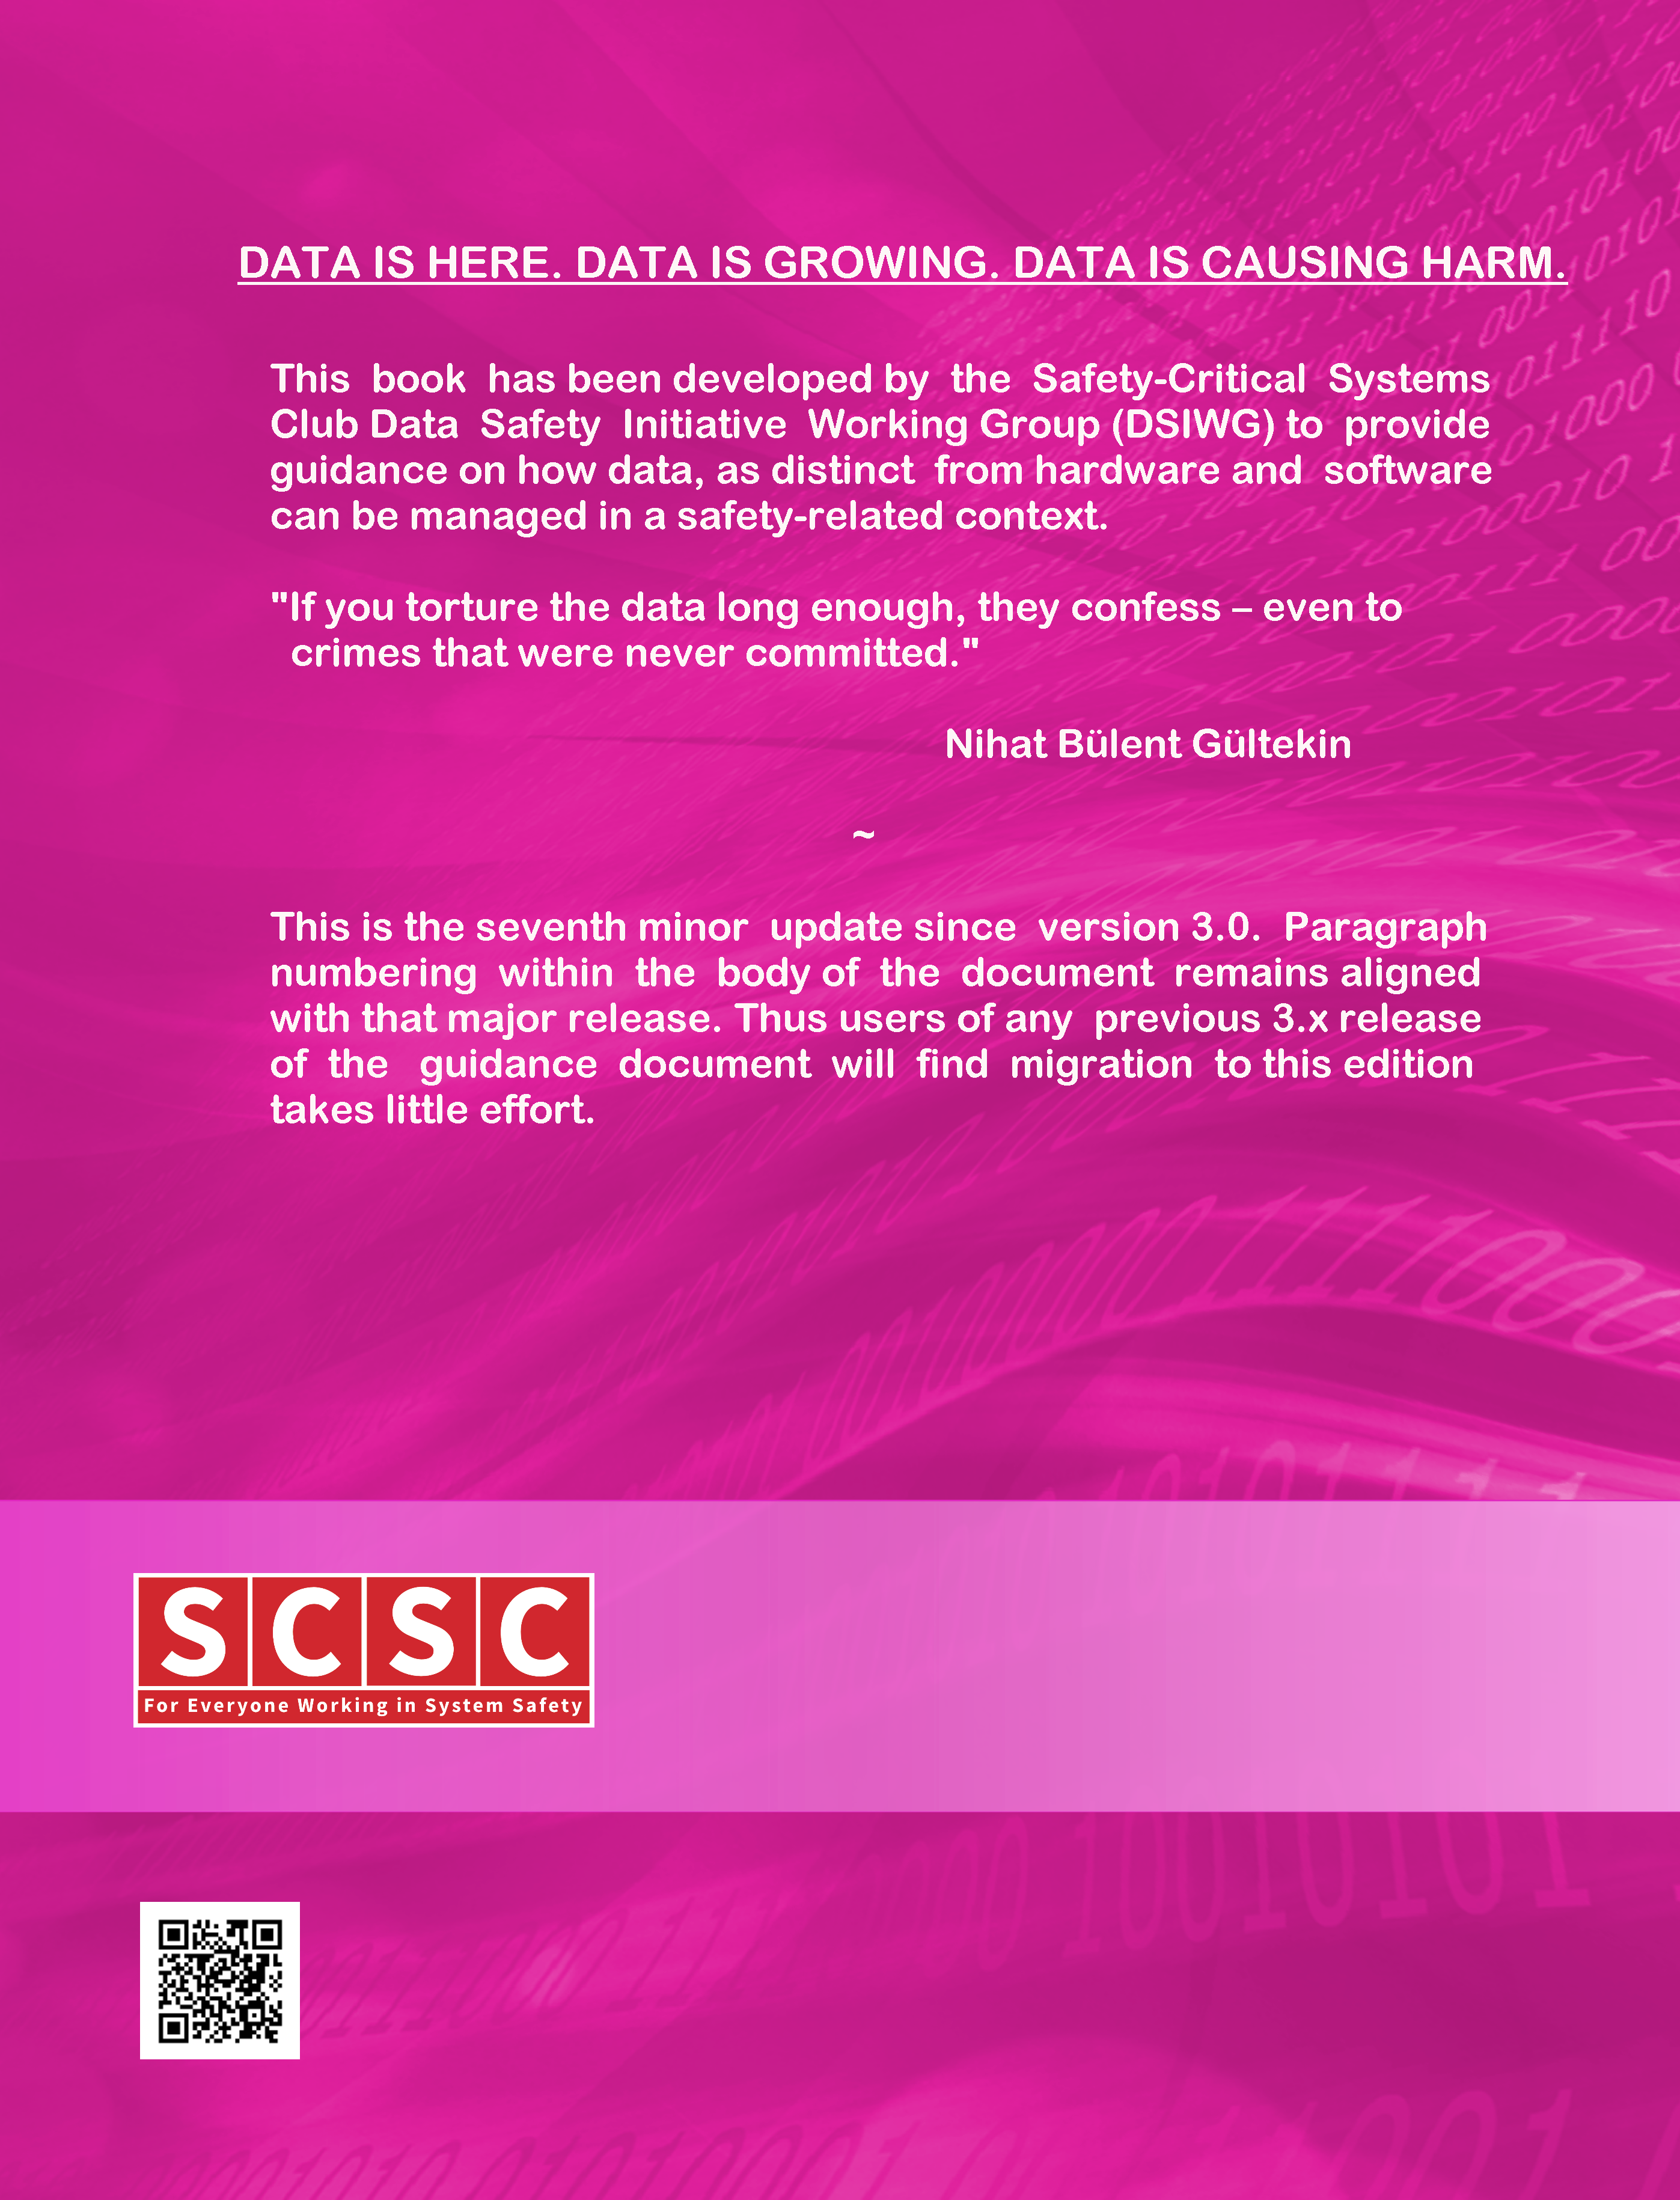
\includepdf{images/back cover.png}
\fi
%

\end{document}